\documentclass[spanish,a4paper,11pt,twoside]{report}

%%%%%%%%%%%%%%%%%%%%%%%%%%%%%%%%%%%%%%%%%%%%%%%%%%%%%%%%%%%%%%%%%%%%%%%%%%%%%%%
\usepackage[dvips]{graphicx}
%\usepackage{graphicx}
%\usepackage{graphicsx}
%\usepackage[dvips]{graphics}
\usepackage[dvips]{epsfig}
\usepackage[latin1]{inputenc}
\usepackage[spanish]{babel}
\usepackage{alltt}
\usepackage{templates/algorithm}
\usepackage{templates/algorithmic}
\usepackage{templates/multirow}
%\usepackage{hyperref}




%%%%%%%%%%%%%%%%%%%%%%%%%%%%%%%%%%%%%%%%%%%%%%%%%%%%%%%%%%%%%%%%%%%%%%%%%%%%%%%

\newcommand{\SONY}{{\sc Sony}}
\newcommand{\MICROSOFT}{{\sc Microsoft}}
\newcommand{\GCC}{\textsf{\textsc{G}CC}}
\newcommand{\INTEL}{\textsf{\textsc{I}ntel}}

%%% Traducimos el pseudocodigo
\renewcommand{\algorithmicwhile}{\textbf{mientras}}
\renewcommand{\algorithmicend}{\textbf{fin}}
\renewcommand{\algorithmicdo}{\textbf{hacer}}
\renewcommand{\algorithmicif}{\textbf{si}}
\renewcommand{\algorithmicthen}{\textbf{entonces}}
\renewcommand{\algorithmicrepeat}{\textbf{repetir}}
\renewcommand{\algorithmicuntil}{\textbf{hasta que}}
\renewcommand{\algorithmicelse}{\textbf{en otro caso}}
\renewcommand{\algorithmicfor}{\textbf{para}}

%\newcommand{\RETURN}{\textbf{retornar} }
\newcommand{\RET}{\STATE \textbf{retornar} }
\newcommand{\TO}{\textbf{hasta} }
\newcommand{\AND}{\textbf{y} }
\newcommand{\OR}{\textbf{o} }

%%%%%%%%%%%%%%%%% Creamos un entorno para listar c�digo fuente %%%%%%%%%%%%%%%
\newenvironment{sourcecode}
{\begin{list}{}{\setlength{\leftmargin}{1em}}\item\scriptsize\bfseries}
{\end{list}}

\newenvironment{littlesourcecode}
{\begin{list}{}{\setlength{\leftmargin}{1em}}\item\tiny\bfseries}
{\end{list}}

\newenvironment{summary}
{\par\noindent\begin{center}\textbf{Abstract}\end{center}\begin{itshape}\par\noindent}
{\end{itshape}}

\newenvironment{keywords}
{\begin{list}{}{\setlength{\leftmargin}{1em}}\item[\hskip\labelsep \bfseries Keywords:]}
{\end{list}}

\newenvironment{palabrasClave}
{\begin{list}{}{\setlength{\leftmargin}{1em}}\item[\hskip\labelsep \bfseries Palabras clave:]}
{\end{list}}


%%%%%%%%%%%%%%%%%%%%%%%%%%%%%%%%%%%%%%%%%%%%%%%%%%%%%%%%%%%%%%%%%%%%%%%%%%%%%%%
% Format
%%%%%%%%%%%%%%%%%%%%%%%%%%%%%%%%%%%%%%%%%%%%%%%%%%%%%%%%%%%%%%%%%%%%%%%%%%%%%%%

\topmargin -4 mm
%\topmargin -21 mm
%\headheight 10 mm
%\headsep 10 mm

%\textheight 229 mm
%\textheight 246 mm

%\oddsidemargin -5.4 mm
%\evensidemargin -5.4 mm
\oddsidemargin 5 mm
\evensidemargin 5 mm

%\oddsidemargin -3 mm
%\evensidemargin -3 mm

%\textwidth 17 cm
\textwidth 15 cm
%\columnsep 10 mm

\input{amssym.def}

%%%%%%%%%%%%%%%%%%%%%%%%%%%%%%%%%%%%%%%%%%%%%%%%%%%%%%%%%%%%%%%%%%%%%%%%%%%%%%%

\begin{document}

%%%%%%%%%%%%%%%%%%%%%%%%%%%%%%%%%%%%%%%%%%%%%%%%%%%%%%%%%%%%%%%%%%%%%%%%%%%%%%%
% First Page 
%%%%%%%%%%%%%%%%%%%%%%%%%%%%%%%%%%%%%%%%%%%%%%%%%%%%%%%%%%%%%%%%%%%%%%%%%%%%%%%

\pagestyle{empty}
\thispagestyle{empty}


\newcommand{\HRule}{\rule{\linewidth}{1mm}}
\setlength{\parindent}{0mm}
\setlength{\parskip}{0mm}
\vspace*{\stretch{1}}

\begin{center}
\includegraphics[width=0.2\textwidth]{images/logotipo-secundario-ULL}\\[0.25cm]
\end{center}

\HRule
\begin{center}
        {\Huge Series de Polinomio de Taylor} \\[2.5mm] 
        {\Huge Cos(x)} \\[2.5mm]
        {\Large Sergio \'Alvarez Fern\'andez\\
        Cirilo Fleitas Rufino\\
        Rayco Hern\'andez Delgado} \\[5mm]
        {\Large \textit{Grupo ($2H$) }} \\[5mm]


        {\em T\'ecnicas Experimentales. $1^{er}$ curso. $2^{do}$ semestre} \\[5mm]
        Lenguajes y Sistemas Inform\'aticos \\[5mm]
        Facultad de Matem\'aticas \\[5mm]
        
        Universidad de La Laguna \\
\end{center}
\HRule
\vspace*{\stretch{2}}
\begin{center}
  La Laguna, \today 
\end{center}

%%%%%%%%%%%%%%%%%%%%%%%%%%%%%%%%%%%%%%%%%%%%%%%%%%%%%%%%%%%%%%%%%%%%%%%%%%%%%%%

%%%%%%%%%%%%%%%%%%%%%%%%%%%%%%%%%%%%%%%%%%%%%%%%%%%%%%%%%%%%%%%%%%%%%%%%%%%%%%%
%\newpage{\pagestyle{empty}\cleardoublepage}

\pagestyle{myheadings} %my head defined by markboth or markright
% No funciona bien \markboth sin "twoside" en \documentclass, pero al
% ponerlo se dan un mont�n de errores de underfull \vbox, con lo que no se
% ha puesto.
\markboth{}{}

%%%%%%%%%%%%%%%%%%%%%%%%%%%%%%%%%%%%%%%%%%%%%%%%%%%%%%%%%%%%%%%%%%%%%%%%%%%%%%%
%Numeracion en romanos
\renewcommand{\thepage}{\arabic{page}}
\setcounter{page}{1}

%%%%%%%%%%%%%%%%%%%%%%%%%%%%%%%%%%%%%%%%%%%%%%%%%%%%%%%%%%%%%%%%%%%%%%%%%%%%%%%

1\tableofcontents

%%%%%%%%%%%%%%%%%%%%%%%%%%%%%%%%%%%%%%%%%%%%%%%%%%%%%%%%%%%%%%%%%%%%%%%%%%%%%%%
%\newpage{\pagestyle{empty}\cleardoublepage}

\listoffigures

%%%%%%%%%%%%%%%%%%%%%%%%%%%%%%%%%%%%%%%%%%%%%%%%%%%%%%%%%%%%%%%%%%%%%%%%%%%%%%%
%\newpage{\pagestyle{empty}\cleardoublepage}



%%%%%%%%%%%%%%%%%%%%%%%%%%%%%%%%%%%%%%%%%%%%%%%%%%%%%%%%%%%%%%%%%%%%%%%%%%%%%%%
%\newpage{\pagestyle{empty}\cleardoublepage}

%%%%%%%%%%%%%%%%%%%%%%%%%%%%%%%%%%%%%%%%%%%%%%%%%%%%%%%%%%%%%%%%%%%%%%%%%%%%%%%
%Numeracion a partir del capitulo I


\setlength{\parindent}{5mm}

%%%%%%%%%%%%%%%%%%%%%%%%%%%%%%%%%%%%%%%%%%%%%%%%%%%%%%%%%%%%%%%%%%%%%%%%%%%%%%%
\chapter{Motivaci�n y objetivos}
\label{chapter:obj}

%%%%%%%%%%%%%%%%%%%%%%%%%%%%%%%%%%%%%%%%%%%%%%%%%%%%%%%%%%%%%%%%%%%%%%%%%%%%%
% Chapter 1: Motivaci\'on y Objetivos 
%%%%%%%%%%%%%%%%%%%%%%%%%%%%%%%%%%%%%%%%%%%%%%%%%%%%%%%%%%%%%%%%%%%%%%%%%%%%%%%

El objetivo de este trabajo ha sido desarrollar un experimento, para evaluar la serie del polinomio de Taylor de una funci\'on concreta. En nuestro caso el cos(x). Para ello hemos desarrollado un programa en Python, que a partir de recibir varias cotas superiores del error (resto de Taylor) calcula el polinomio de Taylor y lo muestra por pantalla.
Tambi\'en hemos creado un programa para que nos represente en una gr\'afica los polinomios de Taylor anteriormente hallados junto con el cos(x). Y otra gr\'afica que muestra el tiempo empleado en calcular cada polinomio y mostrarlo.

%---------------------------------------------------------------------------------


%%%%%%%%%%%%%%%%%%%%%%%%%%%%%%%%%%%%%%%%%%%%%%%%%%%%%%%%%%%%%%%%%%%%%%%%%%%%%%%

\chapter{Fundamentos te�ricos}
\label{chapter:teo}

%%%%%%%%%%%%%%%%%%%%%%%%%%%%%%%%%%%%%%%%%%%%%%%%%%%%%%%%%%%%%%%%%%%%%%%%%%%%%%%
% Chapter 2: Fundamentos Te\'oricos 
%%%%%%%%%%%%%%%%%%%%%%%%%%%%%%%%%%%%%%%%%%%%%%%%%%%%%%%%%%%%%%%%%%%%%%%%%%%%%%%

%++++++++++++++++++++++++++++++++++++++++++++++++++++++++++++++++++++++++++++++

En c\'alculo, el teorema de Taylor, recibe su nombre del matem\'atico brit\'anico Brook Taylor, quien lo enunci\'o con mayor generalidad en 1712, aunque previamente James Gregory lo hab\'ia descubierto en 1671. Este teorema permite obtener aproximaciones polin\'omicas de una funci\'on en un entorno de cierto punto en que la funci\'on sea diferenciable. Adem\'as el teorema permite acotar el error obtenido mediante dicha estimaci\'on.

%++++++++++++++++++++++++++++++++++++++++++++++++++++++++++++++++++++++++++++++

\section{Teorema de Taylor}
\label{2:sec:1}
Este teorema permite aproximar una funci\'on derivable en el entorno reducido alrededor de un punto $a \in \mbox {(a, d)}$ mediante un polinomio cuyos coeficientes dependen de las derivadas de la funci\'on en ese punto. M\'as formalmente, si $\ n \ge 0$ es un entero y \ f una funci\'on que es derivable \ n veces en el intervalo cerrado [\ a, \ x] y \ n+1 veces en el intervalo abierto (\ a, \ x), entonces se cumple que:

(1a)
  \[f(x) = f(a)
  + \frac{f'(a)}{1!}(x - a)
  + \frac{f^{(2)}(a)}{2!}(x - a)^2
  + \cdots
  + \frac{f^{(n)}(a)}{n!}(x - a)^n
  + R_n(f)\]

O en forma compacta

(1b) \[f(x) = \sum_{k=0}^n \frac{f^{(k)}(a)}{k!}(x - a)^k + R_n(f)\]

Donde $\ k!$ denota el factorial de $\ k, y R_n(f)\,$ es el resto, t\'ermino que depende de \ x y es peque�o si \ x est\'a pr\'oximo al punto \ a. Existen dos expresiones para \ R que se mencionan a continuaci\'on:

(2a)
\[R_n(f) = \frac{f^{(n+1)}(\xi)}{(n+1)!} (x-a)^{n+1}\]

donde \ a y \ x, pertenecen a los n\'umeros reales, $\ n$ a los enteros y $\ \xi$ es un n\'umero real entre \ a y \ x:

(2b)
\[R_n(f) = \int_a^x \frac{f^{(n+1)} (t)}{n!} (x - t)^n \, dt\]

Si $R_n(f)\,$ es expresado de la primera forma, se le denomina T\'ermino complementario de Lagrange, dado que el Teorema de Taylor se expone como una generalizaci\'on del Teorema del valor medio o Teorema de Lagrange, mientras que la segunda expresi\'on de R muestra al teorema como una generalizaci\'on del Teorema fundamental del c\'alculo integral.

Para algunas funciones $\ f(x),$ se puede probar que el resto, $\ R_n(f),$ se aproxima a cero cuando $\ n$ se acerca al $\infty$; dichas funciones pueden ser expresadas como series de Taylor en un entorno reducido alrededor de un punto $\ a$ y son denominadas funciones anal\'iticas.

El teorema de Taylor con $\ R_n(f)$ expresado de la segunda forma es tambi\'en v\'alido si la funci\'on $\ f$ tiene n\'umeros complejos o valores vectoriales. Adem\'as existe una variaci\'on del teorema de Taylor para funciones con m\'ultiples variables.

 
 
 
 
 
 
  En \LaTeX{}~\cite{Lamport:LDP94} es sencillo escribir expresiones
matem\'aticas como $a=\sum_{i=1}^{10} {x_i}^{3}$
y deben ser escritas entre dos s\'imbolos \$.
Los super\'indices se obtienen con el s\'imbolo \^{}, y
los sub\'indices con el s\'imbolo \_.
Por ejemplo: $x^2 \times y^{\alpha + \beta}$.


\subsection{Demostraci\'on}

La demostraci\'on de la f�rmula (1a), con el resto de la forma (2a), se sigue trivialmente del teorema de Rolle aplicado a la funci�n:

\[F(y) = f(x) - f(y) - \frac{f'(y)}{1!}(x-y) - \dots - \frac{f^{(n)}(y)}{n!}(x-y)^n\]

Un c\'alculo rutinario permite ver que la derivada de esta funci\'on cumple que:

\[F'(y) = -\frac{f^{(n+1)}(y)}{n!}(x-y)^n\]

Se define ahora la funci\'on G como:

\[G(y) = F(y) - \left(\frac{x-y}{x-a}\right)^{n+1}F(a)\] 

Es evidente que esta funci\'on cumple $\scriptstyle G(a) = G(x) = 0$, y al ser esta funci\'on diferenciable, por el teorema de Rolle se sigue que:

\[\exists \xi\in(x,a): G'(\xi) = 0\]

Y como:

\[0 = G'(\xi) = F'(\xi)+(n+1) \frac{(x-\xi)^n}{(x-a)^{n+1}}F(a)\]

Se obtiene finalmente que:

\[F(a)=\frac{f^{(n+1)}(\xi)}{(n+1)!}(x-a)^{n+1}\]

Y sustituyendo en esta f\'ormula la definici\'on de F(a), queda precisamente la f\'ormula (1a) con la forma del resto (2a).

\subsection{Propiedades}

 $\alpha,\beta \in\mbox{R}$, $f$ y $g$ funciones.\\
 \\
(1)
$T_n(\alpha f+\beta g)=\alpha T_n(f)+\beta T_n(g)$\\ \\
(2)
$T_n( f\cdot g)= T_n(f)\cdot T_n(g)-${t\'erminos de orden $> n$}\\ \\
(3)
${\displaystyle T_n(f/g)=\frac{T_n(f)}{T_n(g)} }$ "haciendo divisi\'on larga hasta $n$"\\ \\
(4)
$T_n( f\circ g)= T_n(f)\circ T_n(g)-${t\'erminos de orden $> n$}\\ \\
(5)
$[T_n(f)]'=T_{n-1}(f')$\\ \\
(6)
${\displaystyle \int_a^x T_n(f)(t) dt= T_{n+1}(\int_a^x)f(t) dt }$\\ \\
(6)'
${\displaystyle \int T_n(f) =T_{n+1}(\int f)+K }$,      $K\in\mbox{R}$.\\ \\


\section{Coseno}
\label{2:sec:2}

En trigonometr\'ia el coseno (abreviado cos) de un \'angulo agudo en un tri\'angulo rect\'angulo se define como la raz\'on entre el cateto adyacente a dicho \'angulo y la hipotenusa:

    \[cos(\alpha)={b}/{c}\]
    

En virtud del Teorema de Tales, este n\'umero no depende del tri\'angulo rect\'angulo escogido y, por lo tanto, est\'a bien construido y define una funci\'on del \'angulo $\alpha$.

\section{Aproximaciones}
\label{3:sec:3}
Es una representaci\'on inexacta que, sin embargo, es suficientemente fiel como para ser \'util. Aunque en matem\'aticas la aproximaci\'on t\'ipicamente se aplica a n\'umeros, tambi\'en puede aplicarse a objetos tales como las funciones matem\'aticas, figuras geom\'etricas o leyes f\'isicas.
 
\subsection{Series de Potencias}


En matem\'aticas, una serie de Taylor es una representaci\'on de una funci\'on como una infinita suma de t\'erminos.
Estos t\'erminos se calculan a partir de las derivadas de la funci\'on para un determinado valor de la variable (respecto de la cual se deriva), lo que involucra un punto espec\'ifico sobre la funci\'on. Si esta serie est\'a centrada sobre el punto cero, se le denomina serie de McLaurin.

Esta representaci\'on tiene tres ventajas importantes:

La derivaci\'on e integraci\'on de una de estas series se puede realizar t\'ermino a t\'ermino, que resultan operaciones triviales.
Se puede utilizar para calcular valores aproximados de la funci\'on.
Es posible demostrar que, si es viable la transformaci\'on de una funci\'on a una serie de Taylor, es la \'optima aproximaci\'on posible.
Algunas funciones no se pueden escribir como serie de Taylor porque tienen alguna singularidad. En estos casos normalmente se puede conseguir un desarrollo en serie utilizando potencias negativas de x (v\'ease Serie de Laurent. Por ejemplo $f(x) = exp(-1/x�)$ se puede desarrollar como serie de Laurent.



%%%%%%%%%%%%%%%%%%%%%%%%%%%%%%%%%%%%%%%%%%%%%%%%%%%%%%%%%%%%%%%%%%%%%%%%%%%%%%%
\chapter{Procedimiento experimental}
\label{chapter:exp}

%%%%%%%%%%%%%%%%%%%%%%%%%%%%%%%%%%%%%%%%%%%%%%%%%%%%%%%%%%%%%%%%%%%%%%%%%%%%%%%
% Chapter 3: Procedimiento experimental 
%%%%%%%%%%%%%%%%%%%%%%%%%%%%%%%%%%%%%%%%%%%%%%%%%%%%%%%%%%%%%%%%%%%%%%%%%%%%%%%

Para realizar los pertinentes experimentos hemos creado un programa en lenguaje Python, que para cada una de las cotas de error recibidas, halla el t\'ermino en el cual el resto del polinomio de Taylor pasa a ser menor que el error. Una vez hallado el grado del resto utiliza este valor para representar el polinomio de Taylor que es de un grado menos que el grado del resto.
Tambi\'en hemos creado un programa para que nos represente en una gr\'afica los polinomios de Taylor anteriormente hallados junto con el cos(x). Y otra gr\'afica que muestra el tiempo empleado en calcular cada polinomio y mostrarlo.

%++++++++++++++++++++++++++++++++++++++++++++++++++++++++++++++++++++++++++++++
\section{Descripci\'on de los experimentos}
\label{3:sec:1}

Para realizar distintos experimentos debemos cambiar las cotas de error con lo que lograremos que se generen distintos polinomios de Taylor. Y gracias a la representaci\'on gr\'afica podemos ver cuanto se aproximan estos polinomios a la funci\'on cos(x).
Otros experimentos posibles ser\'ian cambiar el valor del centro y tambi\'en cambiar el valor del punto donde debe ser evaluado. En ambos casos con un objetivo similar al primer experimento.
\\ \\ \\ \\ \\ \\ \\ \\ \\ \\ \\ \\ \\ \\

%++++++++++++++++++++++++++++++++++++++++++++++++++++++++++++++++++++++++++++++
\section{Resultados obtenidos}
\label{3:sec:2}
Todos los experimentos fueron realizados para cinco cotas de error, estas son: [0.4789, 0.0456, 0.00005, 0.000000005, 0.000000000007].\\ 

En primer lugar ejecutamos el programa con el centro fijado en el punto 0 y con un valor de 2 para el punto.
\begin{figure}[htb]
\begin{center}
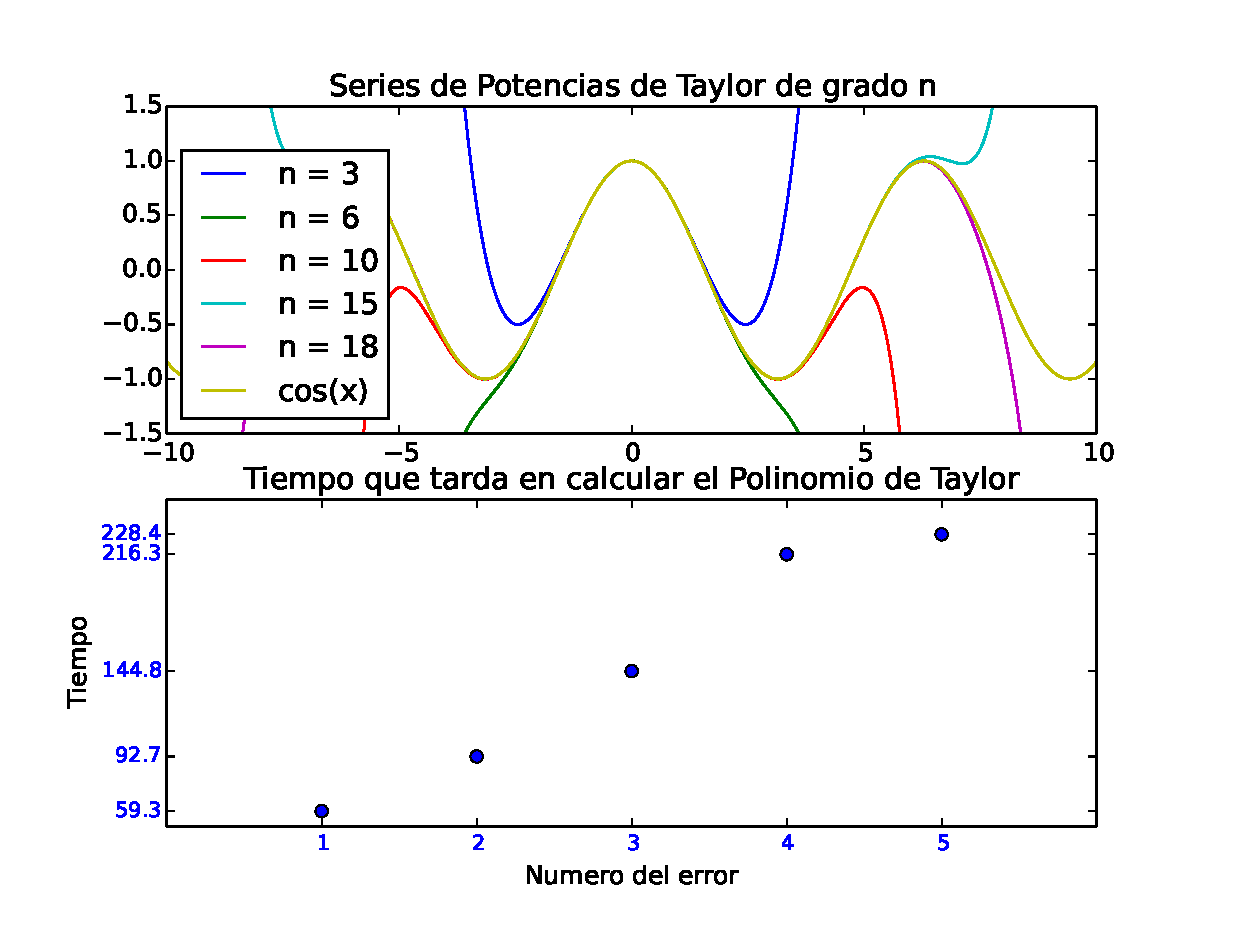
\includegraphics[width=10cm]{Graficas.eps}
\caption{Grafico de Taylor}
\label{fig}
\end{center}
\end{figure}

Podemos ver como cuanto mayor es el grado del polinomio la aproximaci\'on al coseno es mejor.\\ 

En segundo lugar hemos ejecutado el programa con el centro fijado en el punto 5 y con un valor de 2 para el punto.
\begin{figure}[htb]
\begin{center}
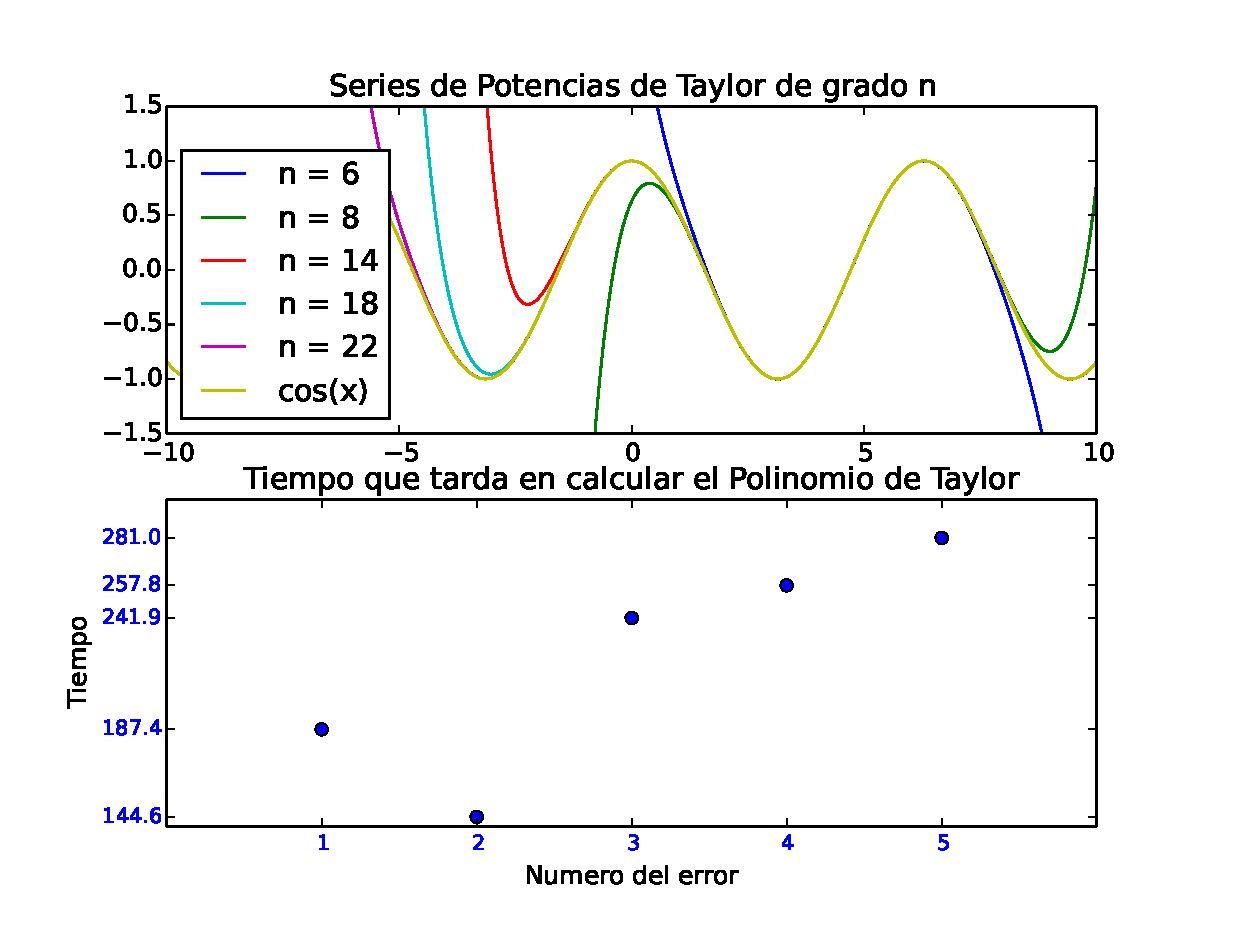
\includegraphics[width=10cm]{images/Graficascentro5.eps}
\caption{Valor del centro 5}
\label{fig}
\end{center}
\end{figure}
\\ \\ \\ \\ \\ \\ \\ \\ \\ \\ \\ \\ \\
En esta gr\'afica podemos ver como el polinomio aproxima al cos(x) pero siendo el punto 5 donde m\'as se aproxima dado que es el centro.\\
Por \'ultimo ejecutamos el programa con el centro fijado en el punto 0 y con un valor de 10 para el punto.
\begin{figure}[htb]
\begin{center}
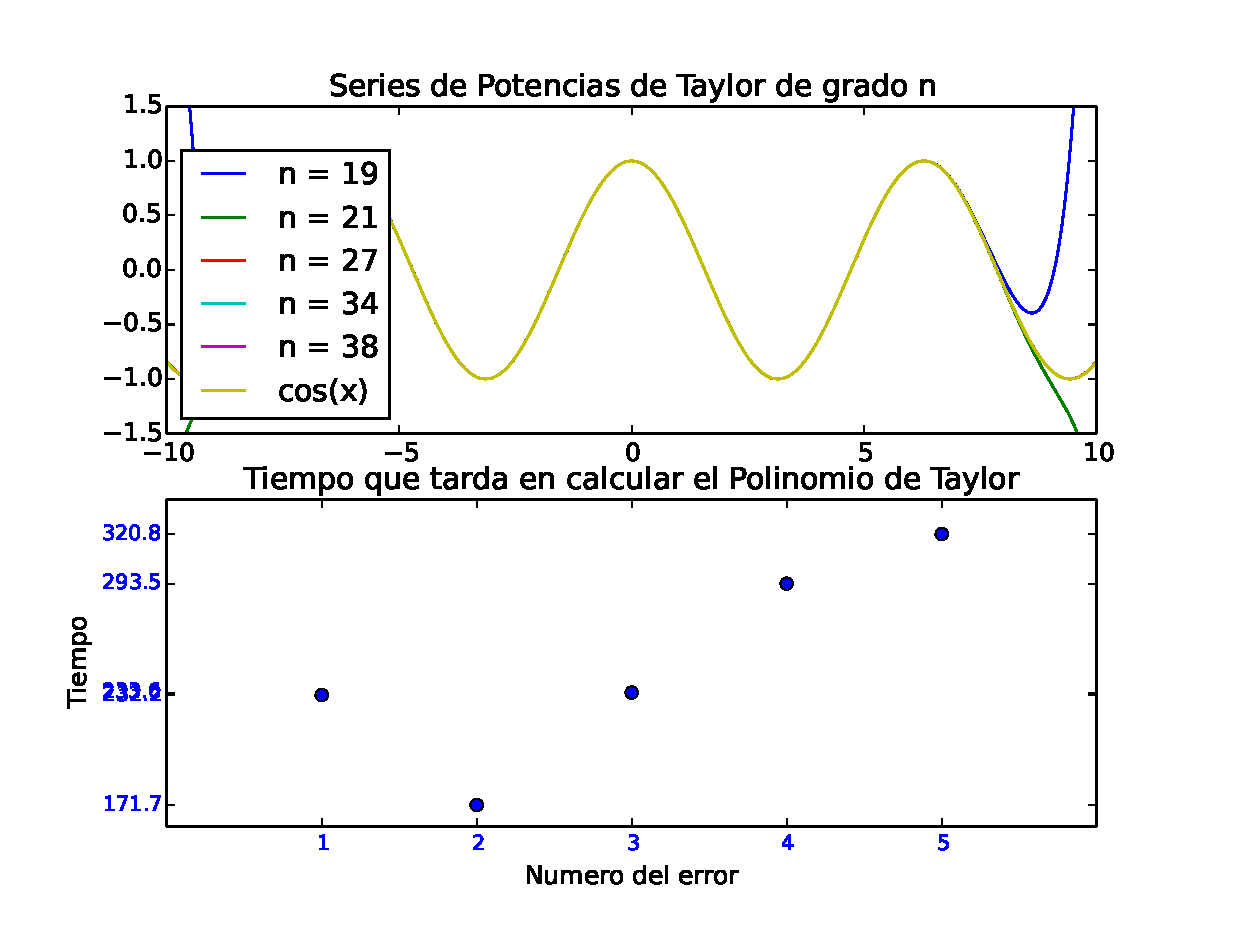
\includegraphics[width=10cm]{images/Graficas10.eps}
\caption{Valor del punto 10}
\label{fig}
\end{center}
\end{figure}

%%%%%%%%%%%%%%%%%%%%%%%%%%%%%%%%%%%%%%%%%%%%%%%%%%%%%%%%%%%%%%%%%%%%%%%%%%%%%%%
\chapter{Conclusiones}
\label{chapter:conclusiones}

%%%%%%%%%%%%%%%%%%%%%%%%%%%%%%%%%%%%%%%%%%%%%%%%%%%%%%%%%%%%%%%%%%%%%%%%%%%%%
% Chapter 4: Conclusiones y Trabajos Futuros 
%%%%%%%%%%%%%%%%%%%%%%%%%%%%%%%%%%%%%%%%%%%%%%%%%%%%%%%%%%%%%%%%%%%%%%%%%%%%%%%

El desarrollo en series de Taylor de una funci\'on en un punto permite obtener resultados con una gran aproximaci\'on al valor real del la funci\'on en ese punto. Tiene muchas aplicaciones te\'oricas adem\'as de las pr\'acticas.


%%%%%%%%%%%%%%%%%%%%%%%%%%%%%%%%%%%%%%%%%%%%%%%%%%%%%%%%%%%%%%%%%%%%%%%%%%%%%%%

%%%%%%%%%%%%%%%%%%%%%%%%%%%%%%%%%%%%%%%%%%%%%%%%%%%%%%%%%%%%%%%%%%%%%%%%%%%%%%%
\newpage{\pagestyle{empty}\cleardoublepage}
\thispagestyle{empty}
\begin{appendix}

\chapter{C�digo python}
\label{appendix:1}

\section{Programa python para hallar el polinomio de Taylor}
\label{}

\begin{center}
\begin{footnotesize}
\begin{verbatim}

#!/usr/bin/python
import random, sys
from sympy import *
import numpy as np 
import math
import time
import timeit

Errores=[0.4789, 0.0456, 0.00005, 0.000000005, 0.000000000007]
x=2.0
c=0.0
f=(x+c)/2

valor_c = Symbol('c')
valor_a = Symbol('f')
funcion = cos(valor_c)
funcion_ = cos (valor_a)


def fac(n):
  if n == 0:
    return 1
  else:
    return n * fac(n-1)

def MostrarTaylor(c,n):
  for i in range(n + 1):
    derivada = eval(str(diff(funcion,valor_c,i)))
    if (i<1):
     sys.stdout.write((str(derivada)))
    if(i>=1):
     x=Symbol('x')
     a=(derivada*((x-c)**i))
     if (derivada != 0):
       if (derivada<0):	 
        a=-a
        sys.stdout.write((' - '+str(a) +' / '+str (i)+'!'))
       else: 
        sys.stdout.write((' + '+str(a) +' / '+str (i)+'!'))
  print '\n' 
  return 1
  
def graficaTaylor(c,n):
  v=0
  for i in range(n + 1):
    derivada = eval(str(diff(funcion,valor_c,i)))
    if (i<1):
     v=v+derivada
    if(i>=1):
     x=np.arange(-10,10,0.001)
     a=(derivada*((x-c)**i))
     if (derivada != 0):
       v=v+derivada*((x-c)**i)/fac(i) 
  return v

  
def ErrorTaylor(x,c,error):
  i=0
  derivada = eval(str(diff(funcion_,valor_a,i)))
  polinomio = ((derivada/(fac(i)))*((x - c)**i))
  while (abs(polinomio)>=error):
    i+=1
    derivada = eval(str(diff(funcion_,valor_a,i)))
    polinomio = ((derivada/(fac(i)))*((x - c)**i))
  return i

 
if __name__=='__main__':
  for error in Errores:
    n=ErrorTaylor(x,c,error)
    print ('\n %3i iteraciones para dar un error <= %.15f') %(n,error)
    MostrarTaylor(c,n-1)


\end{verbatim}
\end{footnotesize}
\end{center}

\section{Programa para representar graficamente los polinomios hallados}
\label{}

\begin{center}
\begin{footnotesize}
\begin{verbatim}
#!/usr/bin/python
#!encoding: UTF-8

#import pylab as dibujo
import sys
from sympy import *
import math
import time
import timeit

import numpy as np 
import matplotlib.pyplot as plt
import calculotaylor  #programa anterior


n=3



tiempo=[]
xtiempo=[]



graf1= plt.subplot(211)
print"Cargado el   0 por ciento de las Graficas"
i=0
for error in calculotaylor.Errores:
    start=time.time()
    i+=1
    n=calculotaylor.ErrorTaylor(calculotaylor.x,calculotaylor.c,error)
    x1=np.arange(-10,10,0.001)
    y=calculotaylor.graficaTaylor(calculotaylor.c,n)
    plt.plot(x1,y, label= 'n = %d' %(n-1))
    print"Cargado %3d por ciento de las Graficas" %(100*i/(len(calculotaylor.Errores))) # Calcula el % de los datos introducidos en el Grafica, así hace la espera mas amena.
    finish=time.time()-start
    tiempo=tiempo+[finish]
plt.plot(x1,np.cos(x1), label = 'cos(x)')    
plt.title('Series de Potencias de Taylor de grado n')
plt.legend(loc = 3) 
plt.ylim(-1.5,1.5)

for i in range (1,len(tiempo)+1):
  xtiempo=xtiempo+[i]
  
graf2=plt.subplot(212)
plt.title('Tiempo que tarda en calcular el Polinomio de Taylor')
plt.plot(xtiempo,tiempo, 'bo')
plt.xticks(xtiempo, size = 'small', color = 'b')
plt.yticks(tiempo, size = 'small', color = 'b')
plt.xlabel("Numero del error")
plt.ylabel("Tiempo")
plt.xlim(0,(len(tiempo)+1))

plt.savefig("Graficas.eps", dpi=100)
plt.show()


\end{verbatim}
\end{footnotesize}
\end{center}




\end{appendix}

%%%%%%%%%%%%%%%%%%%%%%%%%%%%%%%%%%%%%%%%%%%%%%%%%%%%%%%%%%%%%%%%%%%%%%%%%%%%%%%
\addcontentsline{toc}{chapter}{Bibliograf�a}
\bibliographystyle{plain}


\bibliography{bib/references}
%\nocite{*}

%%%%%%%%%%%%%%%%%%%%%%%%%%%%%%%%%%%%%%%%%%%%%%%%%%%%%%%%%%%%%%%%%%%%%%%%%%%%%%%

\end{document}
